\section{Tools \& Tactics}

\begin{frame}[fragile]{Microsoft Exchange Transport Agent}
    \begin{itemize}
        \item Transport agents let you install custom software that is created by Microsoft, by third-party vendors, or by your organization, on an Exchange server \cite{transMicro}
        \item This software can then process email messages that pass through the transport pipeline
        \item Having a single pipeline means that you can have confidence that every message goes is processed in the same way; however it also means that if an attacker can introduce a transport agent, they have access to \emph{every message}
        \item LightNeuron it's the first malware that uses a Transport Agent for malicious purposes
    \end{itemize}
\end{frame}

\begin{frame}[fragile]{LightNeuron components}
    Two main components comprise LightNeuron: 
    \begin{itemize}
        \item a \emph{Transport Agent} that can process and modify all email messages going through the mail server 
        \item a companion 64-bit \emph{Dynamic Link Library (DLL)} containing most of the malicious code.
    \end{itemize}
\end{frame}


\begin{frame}[fragile]{Turla modus operandi}
    A tipical Turla attack chain involves:
    \begin{enumerate}
        \item \textbf{Initial Reconnissance}, usually a basic first-stage malware or a more powerful one if they deem the victim interesting (Metasploit, Carbon or Gazer). Very specific targets
        \item \textbf{Credential Gathering}, they move laterally on the network to collect accounts, using stealthy communications and periodically creating new accounts for persistence
        \item \textbf{Exfiltration}, using an HTTP/email C\&C channel and SATCOM IP addresses to obfuscate the traffic content and destination. 
    \end{enumerate}
    
\end{frame}

\begin{frame}[fragile]{LightNeuron Attack Chain (MITRE ATT\&CK)}
    % The basis of ATT&CK is the set of individual techniques that represent actions that adversaries 
    % can perform to accomplish objectives. Those objectives are represented by the tactic categories
    % the techniques fall under.
    %
    % tattica = obiettivo
    % tecnica = attacco per raggiugnere obiettivo (sfuttare vulnerabilità)
    
    \begin{enumerate}
        \item[1.] \textbf{Initial Acces \& Privilege Escalation}: Valid Accounts using MITM, spreadpishing emails and watering-hole attacks
        \item[2.] \textbf{Execution}: PowerShell script to install Lightneuron components
        \item[3a.] \textbf{Collection}: Automated Collection of both emails and files
        \item[3b.] \textbf{Command \& Control}: email communication using cryptography and steganography
        \item[3c.] \textbf{Exfiltration}: Automated and Encrypted exfiltration via C\&C interface with optional night scheduling
    \end{enumerate}
\end{frame}

\begin{frame}[fragile]{Initial Access \& Privilege Escalation}
    \begin{itemize}
        \item Valid Accounts T1078: adversaries may steal the credentials of a 
        specific user or service account using Credential Access techniques
         or capture credentials earlier through social engineering \cite{MitreTechniques}
        \item The attackers must have privileged administrative access to 
        the server in order to start the attack chain 
    \end{itemize}
\end{frame}

\begin{frame}[fragile]{Execution}
    \begin{itemize}
        \item PowerShell T1086: a powershell script is executed
        \item The malicious Transport Agent is a 32-bit Windows DLL developed in .NET
        \item The attackers drop this executable in the Exchange folder located in the 
        Program Files folder.  
    \end{itemize}
\end{frame}

\begin{frame}[fragile]{Execution: Transport Agent Installation}
    Once admin priviledge have been obtained, a PowerShell script is executed to 
    register the DLL as a Transport Agent
    \begin{figure}
        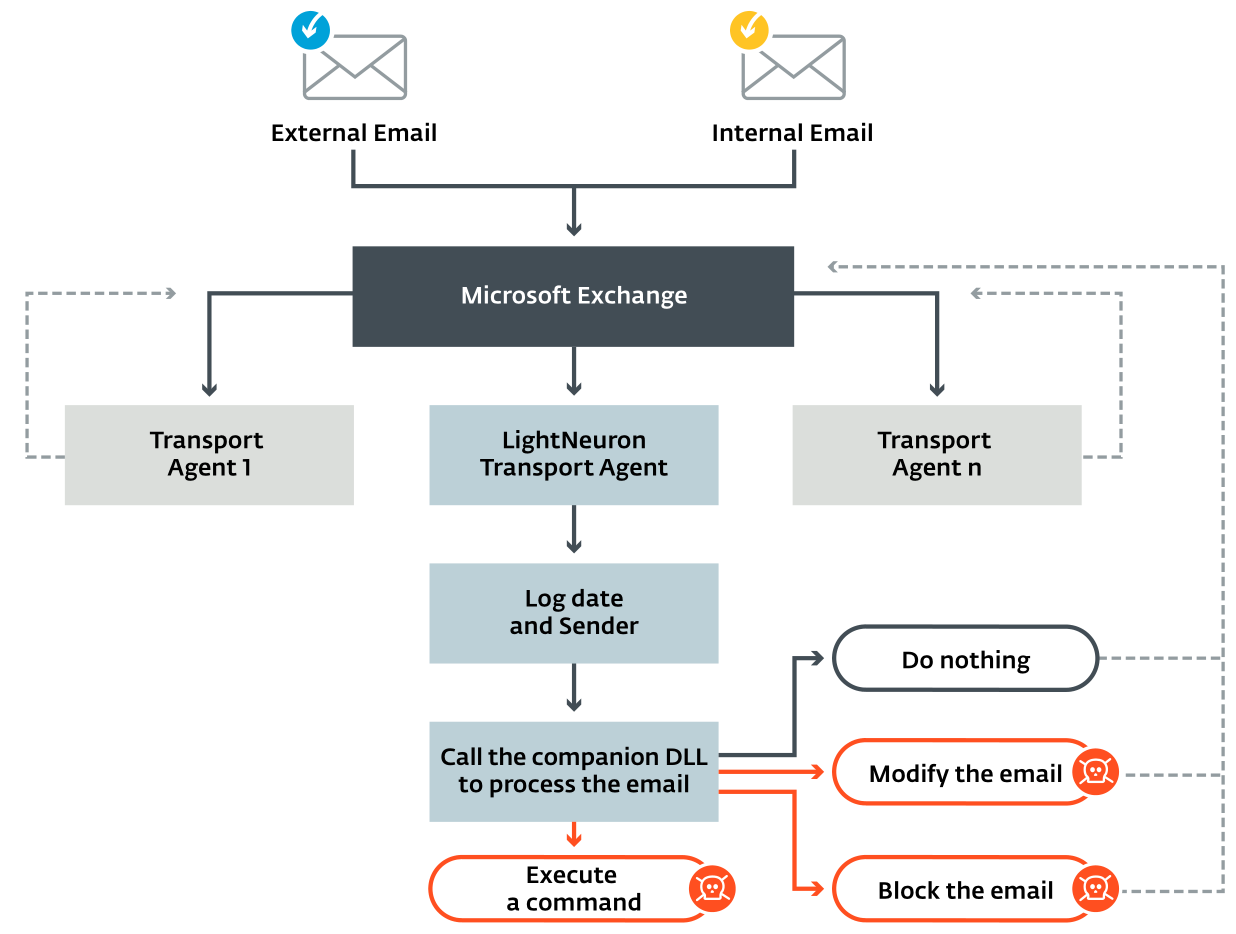
\includegraphics[width=8cm]{figures/transport_agent.PNG}
        \caption{LightNeuron Transport Agent}
    \end{figure}
\end{frame}

\begin{frame}[fragile]{Execution: Companion Dynamic Link Libray}
    \begin{itemize}
        \item The companion DLL is a 64-bit Windows DLL developed in C
        \item When the Transport Agent loads the DLL, 
        the DLL’s main function performs various initialization tasks.
        \item After initail decription operations, it decrypts 
        the configuration file stored in \texttt{\%tmp\%/winmail.dat}; 
        this filename has been chosen to hide their configuration file in plain sight
    \end{itemize}
\end{frame}

\begin{frame}[fragile]{The Configuration Files}
    \begin{itemize}
        \item The configuration file \texttt{winmail.dat} contains various parameters
        \item An interesting one is \texttt{CONFIG\_FILE\_NAME}
        \item Once decrypted, this second configuration file contains the rules used to process the emails.
    \end{itemize}
\end{frame}

\begin{frame}[fragile]{Configuration File Rule System i}
    \begin{itemize}
        \item The second configuration file contains several class nodes, each one corresponding to a different function 
        (aka handler) implemented in the DLL. 
        \item Each class node contains a set of rules describing conditions using the logical operators AND and OR. 
        \item At the end of the file is the mapping of the class names with the name of the functions in the DLL.
    \end{itemize}
    \begin{figure}
        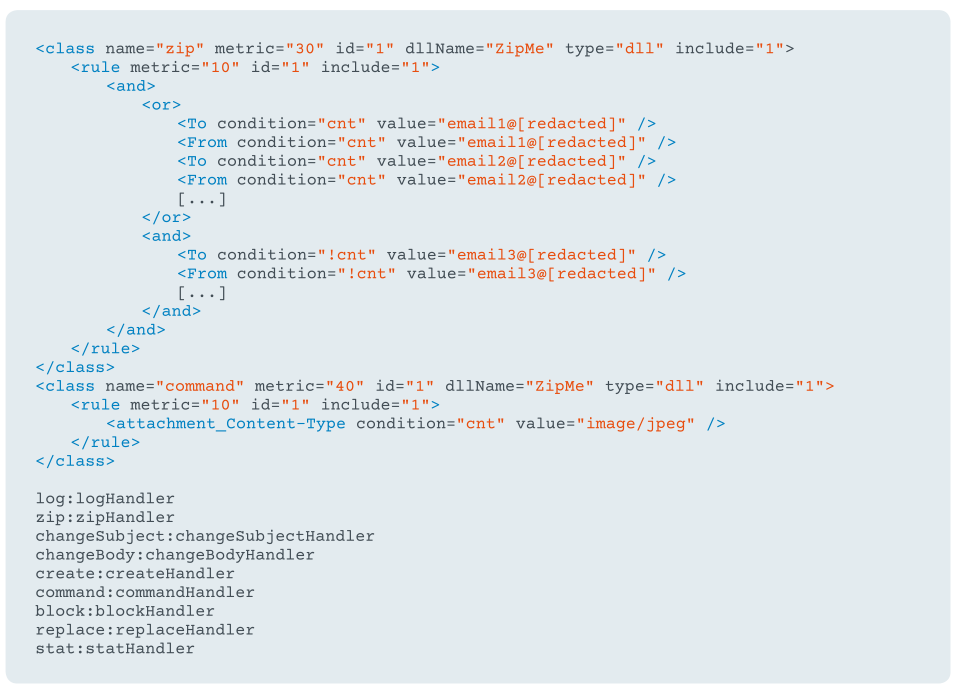
\includegraphics[width=7cm]{figures/rule_file.PNG}
    \end{figure}
\end{frame}

\begin{frame}[fragile]{Configuration File Rule System ii}
    \begin{itemize}
        \item These rules are applied to every email processed by the DLL
        \item This configuration is highly flexible
        \item There are eleven different handlers implemented in the DLL 
    \end{itemize}
    \begin{figure}
        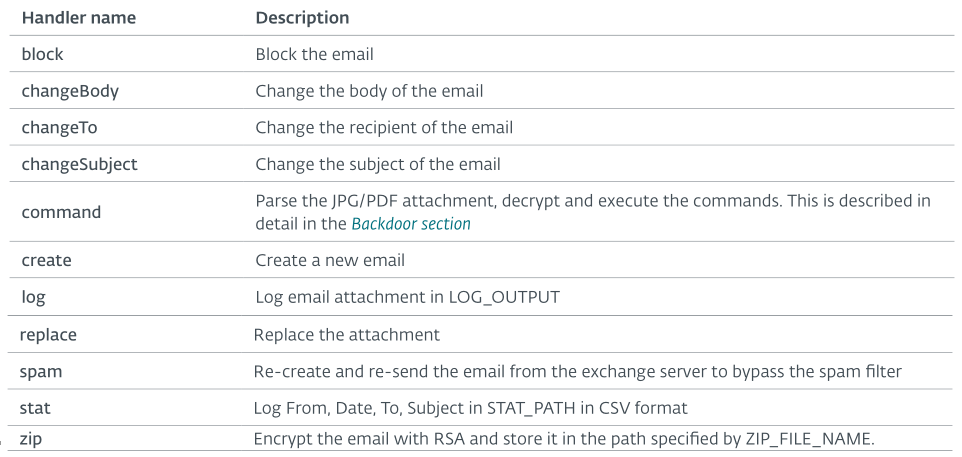
\includegraphics[height=5cm, width=9cm]{figures/handlers.PNG}
        \caption{Description of the handlers implemented in the DLL}
    \end{figure}
\end{frame}

\begin{frame}[fragile]{Collection i}
    \begin{itemize}
        \item Since these rules are applied to every email passing through the transport pipeline, the behavioral characteristics
        of LightNeuron reside in this second configuration file.
        \item MITRE Techniques:
            \begin{itemize}
                \item[] \textbf{Automated Collection} T1119: depending on the configuration, LightNeuron
                can collect the files in a specific path
                \item[] \textbf{Email Collection} T1114: LightNeuron collects all the emails matching 
                one rules specified in its configuration.
            \end{itemize}
    \end{itemize}
\end{frame}

\begin{frame}[fragile]{Collection ii}
    \begin{itemize}
        \item  In every handler definition, the email is in the form
        of a \emph{linked-list} with the different fields parsed (From, To, body, etc.)
        \item The handler can modify this linked-list
        and will return a code corresponding to the action it performed
        \item Then, the Transport Agent interprets this return code to know if it should modify the email, block
        it or execute .NET assembly code
    \end{itemize}
    \begin{figure}
        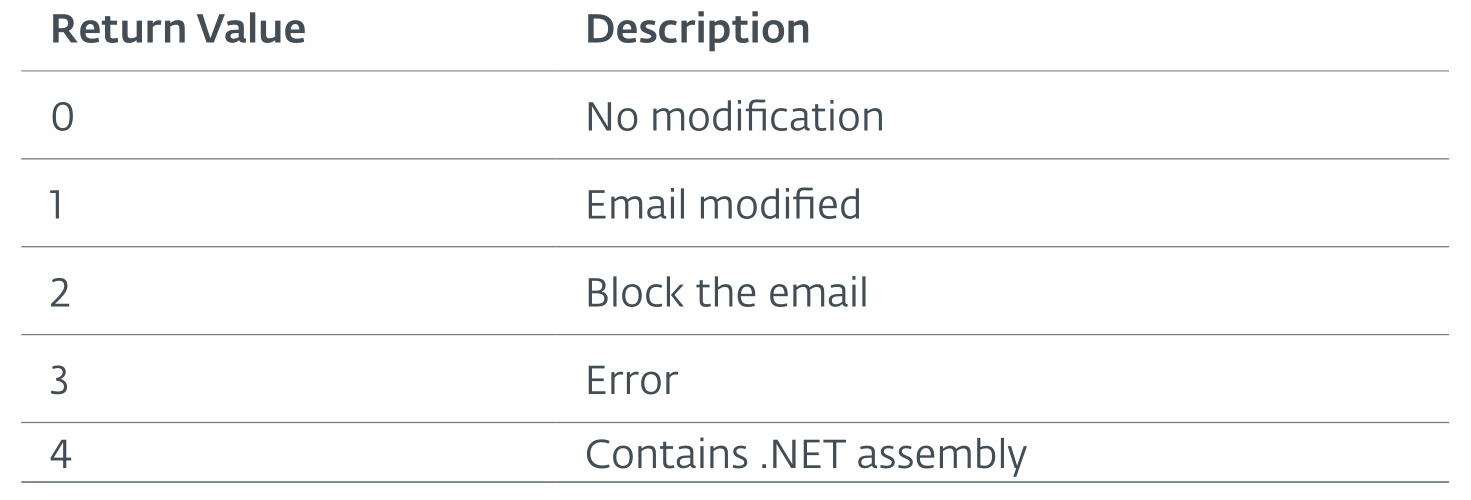
\includegraphics[width=6cm]{figures/return.PNG}
        \caption{Handler return codes and their descriptions}
    \end{figure}
\end{frame}


\begin{frame}[fragile]{Command \& Control and Exfiltration: the backdoor}
    \begin{itemize}
        \item The command handler is actually the implementation of a backdoor controlled by email 
        \emph{(T1071 Standard Application Layer Protocol)}.
        \item It has the following properties:
        \begin{itemize}
            \item[-] Depending on the rules, the commands are hidden in a PDF or a JPG attachment. 
            \item[-] It uses steganography to hide data in PDF documents or JPG pictures. \emph{(T1001 Data Obfuscation)}
        \end{itemize}
        \item One decrypted, the attachment is passed to the routine that reads the blob of data containing the command, aka \emph{container}
    \end{itemize}
\end{frame}

\begin{frame}[fragile]{Command \& Control and Exfiltration: containers i}
    \begin{itemize}
        \item The first four bytes
        are the size of the container and the following bytes are encrypted with AES-256 with a key hardcoded
        in the binary.
        \item Once decrypted, we see the different fields used to store information about the commands to be executed.
        \begin{itemize}
            \item[-] At offset 0x08, the email address to which the result of the command is sent.
            \item[-] At offset 0x1D, the \emph{instruction code}.
            \item[-] At offset 0x25, the first argument of the function that will be called.
        \end{itemize}
    \end{itemize}
    \begin{figure}
        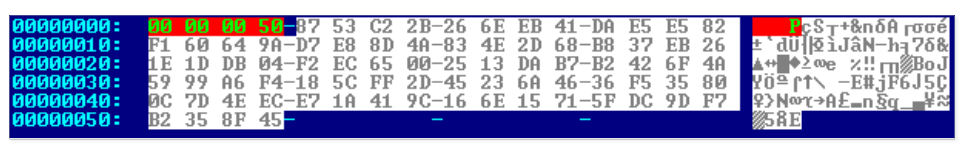
\includegraphics[height=1.6cm, width=9cm]{figures/encr_dump.PNG}
    \end{figure}
    \begin{figure}
        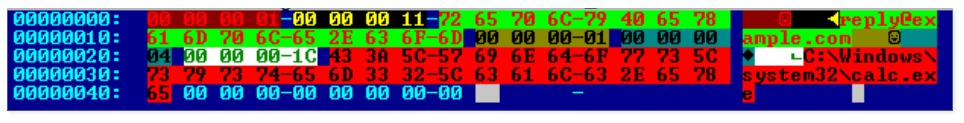
\includegraphics[height=1.6cm, width=9cm]{figures/decr_dump.PNG}
        \caption{Hexadecimal dump of the encrypted (top) decrypted (bottom) container.}
    \end{figure}
\end{frame}


\begin{frame}[fragile]{Command \& Control and Exfiltration: containers ii}
    \begin{itemize}
        \item When processing a container, the backdoor writes the \texttt{CmdId} value to a log file (anti-replay mechanism)
        \item Finally, the command output is encrypted with AES and a PDF document or a JPG image
        \item An email is then created.
    \end{itemize}

    \begin{figure}
        \centering
        \subfloat[List of instruction codes\label{fig:a}]{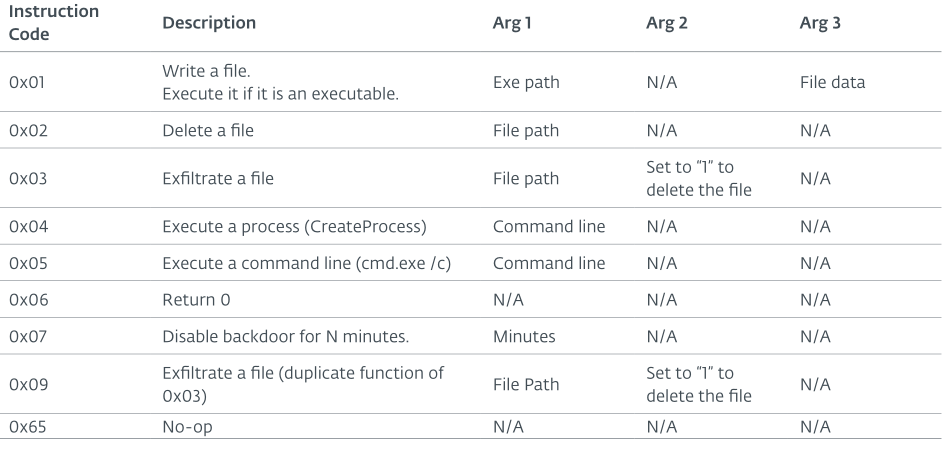
\includegraphics[height=3cm,width=5cm]{figures/istructions.PNG}}\qquad
        \subfloat[Structure of the command container (C-like syntax)\label{fig:b}]{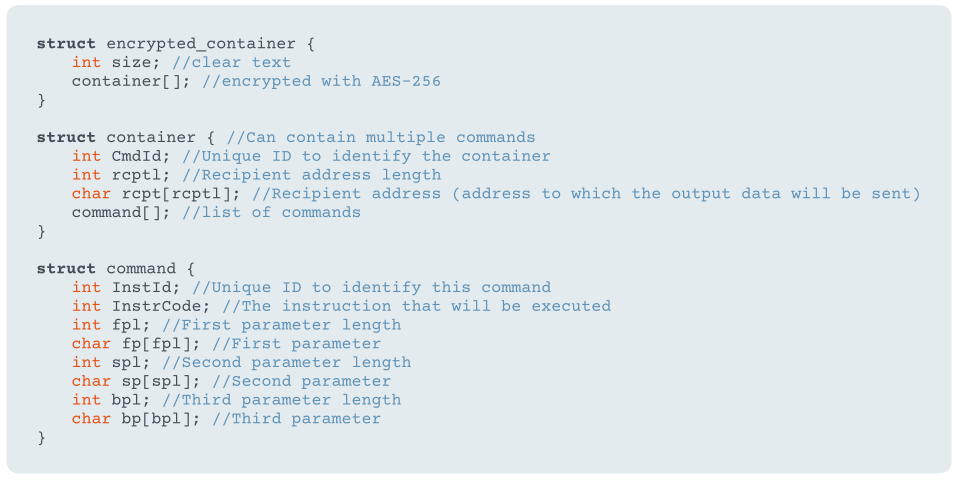
\includegraphics[height=3cm,width=5cm]{figures/command_container.PNG}}
    \end{figure}

\end{frame}

\begin{frame}[fragile]{Command \& Control and Exfiltration: sending the email}
    \begin{itemize}
        \item To send the email, it simply drops it in the folder \\\texttt{<ExchangeInstallFolder>/TransportRoles/PickUp/}
        and the filename starts with \texttt{msg} followed by the result of the \texttt{GetTickCount} function. According to the
        Microsoft documentation \cite{MicroSend}
        \item Moreover exchange does not perform any secutity check on the email sent via this folder
        \item Thus, security solutions will not see the data exfiltrated through LightNeuron, which makes this malware
        very \textbf{stealthy}
    \end{itemize}
\end{frame}

\begin{frame}[fragile]{Command \& Control and Exfiltration: \\Automated and Scheduled Exfiltration}
    \begin{itemize}
        \item If the configuration parameters \texttt{SEND\_TIME} and \texttt{SEND\_AT\_NIGHT} are set, 
        a thread launched by the DLL main function will loop indefinitely.
        \item The exfiltration function loops over the files that match the \texttt{SEND\_FILE} specification
        \item It is possible to include wildcards in the filename specification to match several different files 
        \item Then, for each file, it will send an email containing the file in either a JPG or a PDF attachment
    \end{itemize}
    \begin{figure}
        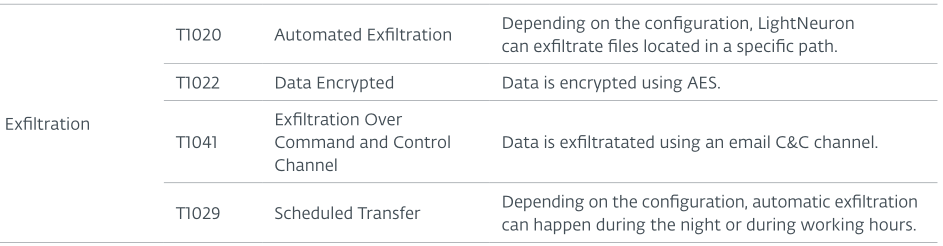
\includegraphics[height=2.3cm, width=9cm]{figures/exfiltration.PNG}
        \caption{Exfiltration MITRE techniquesd used by LightNeuron}
    \end{figure}
\end{frame}
